\section{Exercices Pr\'eparatoires}

\subsection{Exercice 1}
Pour le 2\`eme dispositif, calculez quelle sera l'angle d'\'emission du rayonnement Tcherenkov \'emis dans l’eau par des muons ($m_\mathrm{\mu} = 0.106$\,GeV/$c^2$) de $1.5$\,GeV/$c$ de quantit\'e de mouvement, sachant que l'indice de r\'efraction de l'eau \`a $20^\circ$C est $1.333$.

\ifthenelse{\boolean{showAdditional}}{
\begin{additional}
\begin{align*}
\begin{split}
\beta &= \frac{v}{c} = \frac{pc}{E}\\
 &= \frac{pc}{\sqrt{p^2c^2+m_\mathrm{\mu}^2c^4}}\\
 &= 0.9975\\
\end{split}
\quad
\begin{split}
\cos\Theta_\mathrm{c} &= \frac{1}{\beta n}\\
 \Theta_\mathrm{c} &= \arccos\frac{1}{0.9975\cdot1.33}\\
 &= \boxed{41.2^\circ} 
\end{split}
\end{align*}
\end{additional}
}

\subsection{Exercice 2}
Pour le 1er dispositif, sachant que l'OM est placé à un angle de $45^\circ$ par rapport à la direction d'émission des électrons ($m_\mathrm{e} = 0.511$\,MeV/$c^2$) de la source de strontium, à quel courant faut-il régler le spectromètre pour récolter un maximum de rayonnement Tcherenkov dans l'OM, sachant que l'indice de réfraction du quartz est de $1.478$?\\

Le graphique suivant vous donne la relation entre l'énergie cinétique des électrons et l'intensité du courant.

\begin{figure}[!h]
    \center{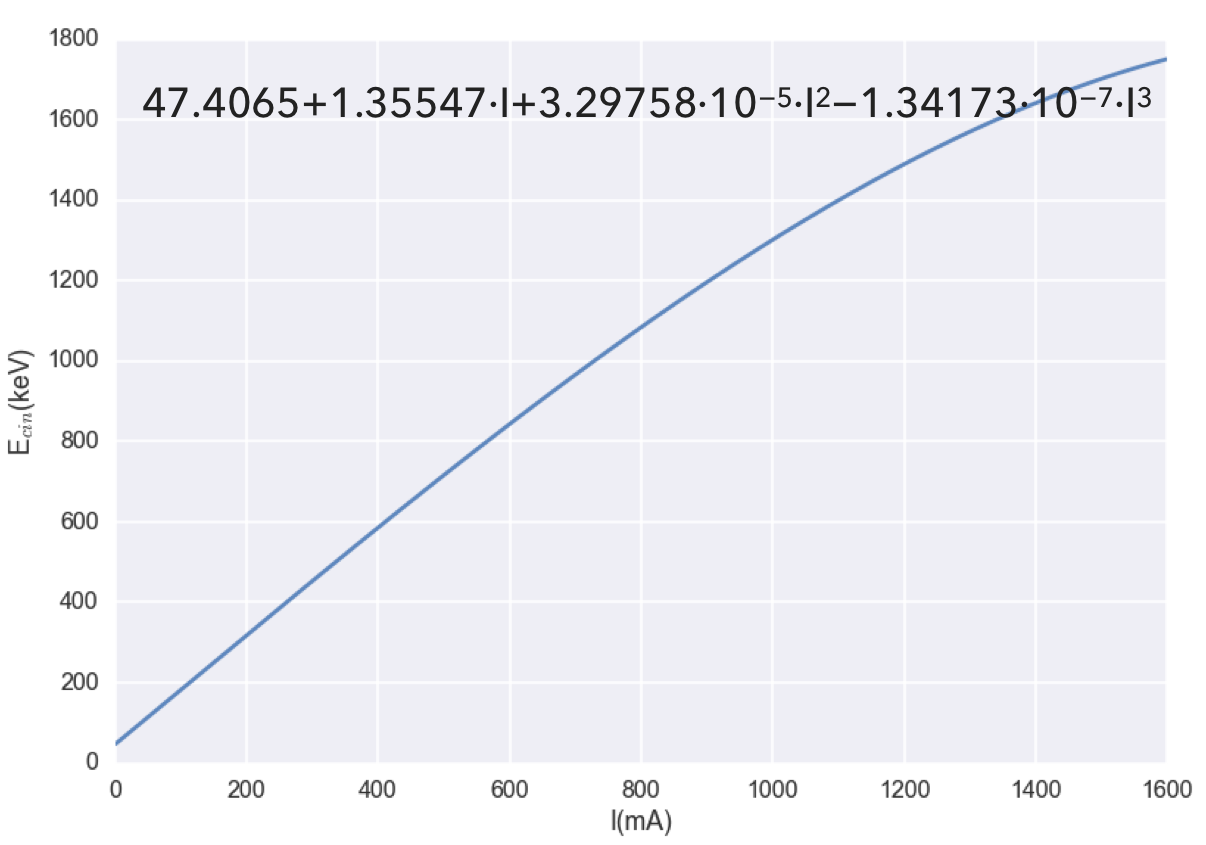
\includegraphics[width=0.5\textwidth]
    {figures/Relation_Ecin_I.png}}
    \caption{\label{fig:spectro} Relation entre l'intensité du courant fourni au spectromètre et l'énergie cinétique des électrons.}
\end{figure}

\ifthenelse{\boolean{showAdditional}}{
\begin{additional}
\begin{align*}
\beta &= \frac{1}{n\cos\Theta_\mathrm{c}} = 0.9568\\
 &= \frac{pc}{E}\\
 &= \frac{\sqrt{E^2-m_\mathrm{e}^2c^4}}{E}\\
 &\\
E &= \sqrt{\frac{m_\mathrm{e}^2c^4}{1 - \beta^2}} = 1.7575\,\mathrm{MeV}\\
E_\mathrm{cin}&=E- m_\mathrm{e}\\
 &= 1.247\,\mathrm{MeV} \\
&\Rightarrow \boxed{I \approx 950\,\mathrm{mA}} \\
\end{align*}
\end{additional}
}

\subsection{Exercice 3}
Pour le 1er dispositif, calculer l'ordre de grandeur du nombre de photons \'emis entre $350$ et $500$\,nm par un 'electron de $1247$\,keV d'\'energie cin\'etique traversant une fen\^etre de quartz de 1\,mm d'\'epaisseur, sachant que pour ce domaine de longueurs d’onde, l'indice de r\'efraction du quartz varie de moins de 1\% et peut \^etre consid\'er'e constant ($1.478$). N\'egliger la perte d'\'energie de l'\'electron dans le quartz.\\ $\alpha = 1/137$

\ifthenelse{\boolean{showAdditional}}{
\begin{additional}
Formule de \emph{Frank-Tamm}:
\begin{align*}
\frac{\mathrm{d}N}{\mathrm{d}x} &= \int_{\lambda_0}^{\lambda_1} \frac{2\pi\alpha z^2}{\lambda^2} \sin^2\Theta_\mathrm{c} \mathrm{d}\lambda\\
&=\frac{\pi}{137}\int_{350\,\mathrm{nm}}^{500\,\mathrm{nm}}\frac{\mathrm{d}\lambda}{\lambda^2}\\
N&=\frac{\pi}{137}\cdot\left(\frac{1}{350\,\mathrm{nm}}-\frac{1}{500\,\mathrm{nm}}\right)\cdot1\,\mathrm{mm}\\
&=\boxed{19.65}
\end{align*}
\end{additional}
}

\subsection{Exercice 4}
En supposant que le diam\`etre du collimateur plac\'e devant la photocathode de l'OM est de 6 cm et qu'il se trouve \`a 17\,cm de la fen\^etre de quartz, combien de photoelectrons l'OM peut-il enregistrer par \'electron de la source, en supposant la transmittance $T$ \`a 90\%, l'efficacit\'e quantique est de $\epsilon_\mathrm{q}=15\%$?

\ifthenelse{\boolean{showAdditional}}{
\begin{additional}
Avec $N_\mathrm{\gamma}^{\mathrm{quartz}}$ trouv\'e avant, on obtient:
\begin{align*}
N_{\mathrm{pe}} &= \epsilon_\mathrm{q} \cdot T \cdot N_\mathrm{\gamma}^{\mathrm{OM}}\\
 &= \epsilon_\mathrm{q} \cdot T \cdot \frac{6\,\mathrm{cm}}{2\pi \cdot 17\,\mathrm{cm} \cdot\sin\Theta_\mathrm{c}} \cdot N_\mathrm{\gamma}^{\mathrm{quartz}}\\
&= \boxed{3.58}
\end{align*}
\end{additional}
}

\pagebreak